\documentclass[final]{fhnwreport}       %[mode] = draft or final
                                        %{class} = fhnwreport, article, 
                                        %          report, book, beamer, standalone
%%---Main Packages-----------------------------------------------------------------------
\usepackage[english, ngerman]{babel}	%Mul­tilin­gual sup­port for LaTeX
\usepackage[T1]{fontenc}				%Stan­dard pack­age for se­lect­ing font en­cod­ings
\usepackage[utf8]{inputenc}				%Ac­cept dif­fer­ent in­put en­cod­ings
\usepackage{lmodern}                    %The newer Font-Set
\usepackage{textcomp}					%LaTeX sup­port for the Text Com­pan­ion fonts
\usepackage{caption}					%Customising captions in floating environments
\usepackage{graphicx} 					%En­hanced sup­port for graph­ics
\usepackage{float}						%Im­proved in­ter­face for float­ing ob­jects
\usepackage{ifdraft}                    %Let you check if the doc is in draft mode
\usepackage{wrapfig}                    %Let wrap text around figures

%%---Useful Packages---------------------------------------------------------------------
\usepackage{color}						%Colour control for LaTeX documents
\usepackage[pdftex,dvipsnames]{xcolor}  %Driver-in­de­pen­dent color ex­ten­sions for LaTeX
\usepackage{csquotes}                   %Simpler quoting with \enquote{}
\usepackage{siunitx} 					%A com­pre­hen­sive (SI) units pack­age
\usepackage{listings}					%Type­set source code list­ings us­ing LaTeX
\usepackage[bottom]{footmisc}			%A range of foot­note op­tions
\usepackage{footnote}					%Im­prove on LaTeX's foot­note han­dling
\usepackage{verbatim}					%Reim­ple­men­ta­tion of and ex­ten­sions to LaTeX ver­ba­tim
\usepackage[textsize=footnotesize]{todonotes} %Mark­ing things to do in a LaTeX doc­u­ment
\usepackage{titling}					%Control over the typesetting of the \maketitle command

%%---Tikz Packages-----------------------------------------------------------------------
\usepackage{standalone}
\usepackage{tikz}
\usepackage{circuitikz}
\usetikzlibrary{arrows}
\usetikzlibrary{calc}
\usetikzlibrary{intersections}

%%---Math Packages-----------------------------------------------------------------------
\usepackage{amsmath}					%AMS math­e­mat­i­cal fa­cil­i­ties for LaTeX
\usepackage{amssymb}					%Type­set­ting symbols (AMS style)
%\usepackage{amstext}
%\usepackage{amsfonts}
%\usepackage{breqn}
\usepackage{array}						%Ex­tend­ing the ar­ray and tab­u­lar en­vi­ron­ments
\usepackage{amsthm}					%Type­set­ting the­o­rems (AMS style)

%%---Table Packages----------------------------------------------------------------------
\usepackage{booktabs}
%\usepackage{vcell}
\usepackage{tabularx}					%Tab­u­lars with ad­justable-width columns
%\usepackage{longtable}
\usepackage{multirow}					%Create tab­u­lar cells span­ning mul­ti­ple rows
\usepackage{makecell}
\usepackage{multicol}					%In­ter­mix sin­gle and mul­ti­ple columns
\usepackage[normalem]{ulem}
\useunder{\uline}{\ul}{}

%%---PDF / Figure Packages---------------------------------------------------------------
\usepackage{pdfpages}					%In­clude PDF doc­u­ments in LaTeX
\usepackage{pdflscape}					%Make land­scape pages dis­play as land­scape
\usepackage{subfig}					    %Fig­ures di­vided into sub­fig­ures

%%---Other Packages----------------------------------------------------------------------
%\usepackage{xargs}                     %De­fine com­mands with many op­tional ar­gu­ments

\lstset{
	aboveskip=1ex,
	backgroundcolor=\color{gray!25},
	basicstyle=\small\ttfamily,
	belowskip=1ex,
	breaklines=true,
	columns=fullflexible,
	framerule=0pt,
	framexrightmargin=0em,
	framexleftmargin=0em,
	numbers=left,
	numberstyle=\footnotesize\sffamily,
	tabsize=2
}

\lstdefinestyle{DOS}
{
	backgroundcolor=\color{black},
	basicstyle=\scriptsize\color{white}\ttfamily
}


%%---Bibliography------------------------------------------------------------------------
\usepackage[style=ieee,urldate=comp,backend=biber]{biblatex}
\addbibresource{literature/bibliography.bib}

%%---Main Settings-----------------------------------------------------------------------
\graphicspath{{./graphics/}}			%Defines the graphicspath
\geometry{twoside=false}				    %twoside=false disables the "bookstyle"
\setlength{\marginparwidth}{2cm}
\overfullrule=5em						%Creates a black rule if text goes over the margins => debugging




%%---User Definitions--------------------------------------------------------------------
%%Tabel-Definitions: (requires \usepackage{tabularx})
\newcolumntype{L}[1]{>{\raggedright\arraybackslash}p{#1}}    %column-width and alignment
\newcolumntype{C}[1]{>{\centering\arraybackslash}p{#1}}
\newcolumntype{R}[1]{>{\raggedleft\arraybackslash}p{#1}}

%%---Optional Package Settings-----------------------------------------------------------
%Listings-Settings: (requires \usepackage{listings}) => Example with Matlab Code
%\lstset{language=Matlab,%
%    basicstyle=\footnotesize\ttfamily,
%    breaklines=false,%
%    morekeywords={switch, case, otherwise},
%    keywordstyle=\color{Blue},%
%    tabsize=2,
%    %morekeywords=[2]{1}, keywordstyle=[2]{\color{black}},
%    identifierstyle=\color{Black},%
%    stringstyle=\color{Purple},
%    commentstyle=\color{Green},%
%    showstringspaces=false,%without this there will be a symbol in the places where there is a space
%    numbers=left,%
%    numberstyle={\tiny \color{black}},% size of the numbers
%    numbersep=9pt, % this defines how far the numbers are from the text
%    %emph=[1]{word1, word2,...},emphstyle=[1]\color{red}
%}							

%Hurenkinder und Schusterjungen verhindern (kein Scherz, Google es)
\clubpenalty10000
\widowpenalty10000
\displaywidowpenalty=10000	


%%---Costum Packages Bachelor Thesis-------------------------------------------
\usepackage{diagbox}

\usepackage{hyperref}
\hypersetup{
    colorlinks=true,
    linkcolor=black,
    filecolor=black,       
    urlcolor=blue,
    citecolor=black,
}			                %loads all packages, definitions and settings
\addbibresource{literature/bibliography.bib}							
\title{Fachbericht}  		        %Project Title
\author{Anklin, Bobst, Horath}      				    %Document Type => Technical Report, ...
\date{\today}          				   %Place and Date

\begin{document}

%%---TITLEPAGE---------------------------------------------------------------------------------
\thispagestyle{empty}
%	\ohead{\includegraphics[scale=0.5]{Bilder/Logo_FHNW.jpg}}
	\begin{figure}
		 \vspace*{-\topskip}\vspace*{-\headsep}
		
\includegraphics[scale=1]{graphics/fhnw_ht_logo_de.pdf}
	\end{figure}
	\begin{center}
		\vspace*{2cm}
		{\huge{\textbf{\thetitle}}}\\
		\vspace*{1cm}
		
		{\huge{Testumgebung und Performancevergleich von Zigbee, Thread und Bluetooth Mesh Netzwerken}}\\
		\vspace*{0.5cm}
		
		{\scshape\Large Bachelor Thesis - \theauthor \\} \Large{\today}
		\vfill
		
		
		\begin{normalsize}
			{\begin{tabbing}
						
					\textbf{Fachcoach:} \hspace{6cm}\= Matthias Meier\\
					\>Manuel Di Cerbo\\
					
					\\[0.4cm]
					
					\textbf{Team:} \>Raffael Anklin \\ \>Robin Bobst \\ \>Cyrill Horath
					\\[0.8cm]
					\textbf{Studiengang:} \>Elektro- und Informationstechnik
					\\[0.8cm]	\textbf{Semester:} \>Frühlingssemester 2020
			\end{tabbing}}
		\end{normalsize}
		\vfill
	\end{center}
\clearpage

%%---ABSTRACT----------------------------------------------------------------------------
\selectlanguage{english}				%ngerman or english
\thispagestyle{empty}
\begin{abstract}
	Among the most popular low power mesh network protocols in free GHz ISM band the three mesh stacks Bluetooth Mesh, ZigBee and Thread are currently competing against each other. The assignment of this bachelor thesis was to build a consistent test framework for all three mesh-networks to benchmark them under realistic conditions. Due to better combability\todo{What ist combability? Is this a Robintypo?}, the nRF52840 SoC from Nordic Semiconductors was the chosen microcontroller for all three network stacks. The benchmark is structured in two parts, a battery powered slave node and a master which is directly connected to a computer. The master node is responsible for controlling the measurement, whereas the slave nodes send benchmark messages to each other. These benchmark messages collect the necessary information to determine latency, RSSI, throughput and active radio time. For a better comparability an apartment house, an apartment and a labor environment were selected as different test benches. The Thread stack results the best in the different test benches. Because of its automatic routing it is able to adapt himself to the environment, as a result the latency of this stack is in every three benches similarly low. Bluetooth Mesh was able to reach the lowest latency with small payload. The ZigBee network stands out with its constant and low latency within one test bench. As a conclusion all of the three networks perform well in case of a home automation. Due to of their own assets and drawbacks it cannot be said this is the best mesh-stack. It depends on the application which mesh network performs the best.
\end{abstract}




%%---TABLE OF CONTENTS-------------------------------------------------------------------
\pagenumbering{Roman}		
\selectlanguage{ngerman}				%ngerman or english
\tableofcontents
\clearpage

%%---TEXT--------------------------------------------------------------------------------
\pagenumbering{arabic}

%%Part 0 Allgemeiner Teil

\clearpage

\section{Einleitung}\label{sec:Einleitung}

\todo[inline]{Allgemeine Einleitung in das Thema und die Arbeit. Die Gliederung des Berichts und die Aufteilung in Total 5 Teile soll erläutert werden --> Leseführung.}

\todo[inline]{Cyrill}
\pagebreak

\clearpage
\section{Hardware Plattform}\label{sec:HardwarePlattform}


\subsection{System on Chip}\label{sec:SystemonChip}

\pagebreak

\clearpage
\section{Point to Point Testinfrastruktur}\label{sec:PointtoPointTestinfrastruktur}



\pagebreak

\clearpage
\section{Projektmanagement}\label{sec:Projektmanagement}




\subsection{Projektaufteilung}\label{subsec:Projektaufteilung}


\subsection{Projektplan}\label{subsec:Projektplan}



\subsection{Risikoanalyse}\label{subsec:Risikoanalyse}


\pagebreak

%%Part 1 Bluetooth Mesh

\vspace*{4cm}
\part{Bluetooth Mesh}\label{part:BluetoothMesh}
Raffael Anklin
\vspace*{\fill}
\clearpage

\section{Einleitung}\label{sec:EinleitungBluetooth}


Bluetooth Mesh ist ein auf dem Bluetooth-Standard aufbauendes Mesh-Netzwerk. Der Standard wurde im Jahr 2017 von der Bluetooth-SIG vorgestellt. Das Ziel des Standards ist es die Reichweite und das Einsatzgebiet von Bluetooth-Geräten zu erweitern. Somit sollen in Zukunft Lichtschalter und Lampen, sowie Sensoren und Aktoren im Heimbereich, Industriebereich und diversen Anwendungsbereichen mittels Bluetooth-Technologie verbunden werden.  \\

\begin{figure}[!htbp]
	\begin{minipage}{0.49\textwidth}
		\centering
		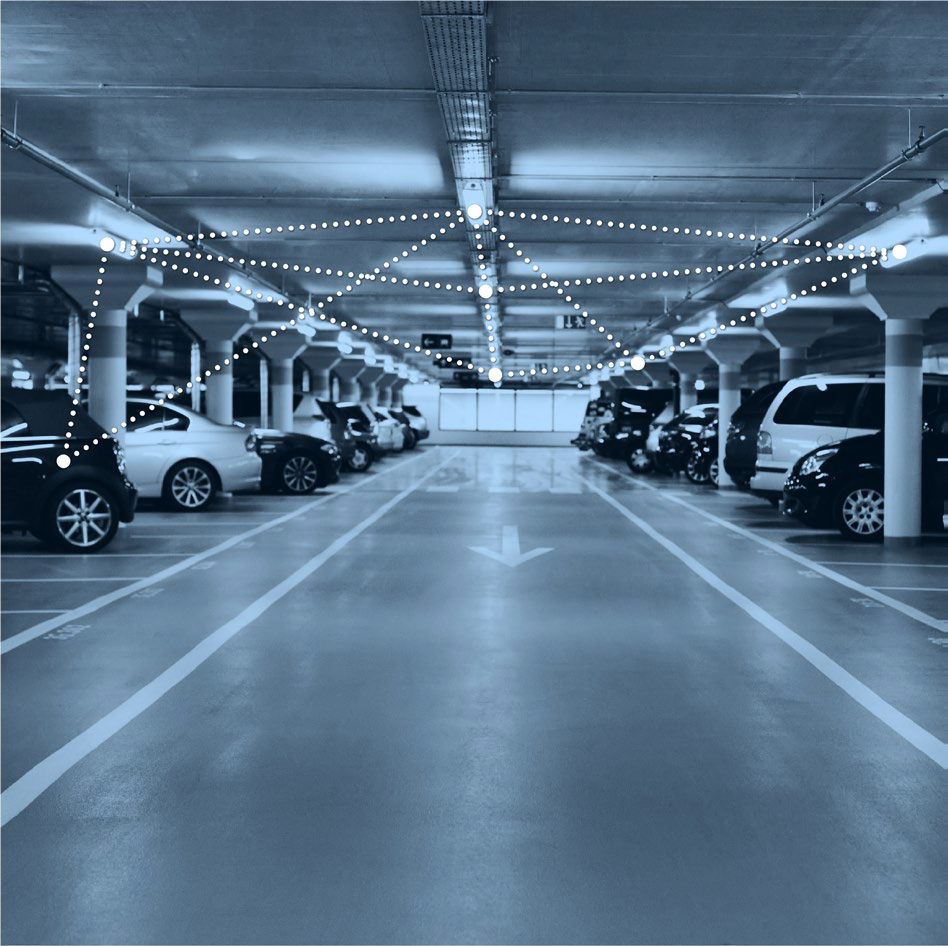
\includegraphics[width=\textwidth]{Bluetooth_Mesh_CarPark_Example.png}
		\caption[Parkhaus mit Bluetooth-Mesh]{Parkhaus mit Bluetooth-Mesh \cite{bluetooth_sig_mesh-technology-overviewpdf_2020}}
		\label{fig:BluetoothMeshParkingExample}
	\end{minipage}
	\begin{minipage}{0.49\textwidth}
		\centering
		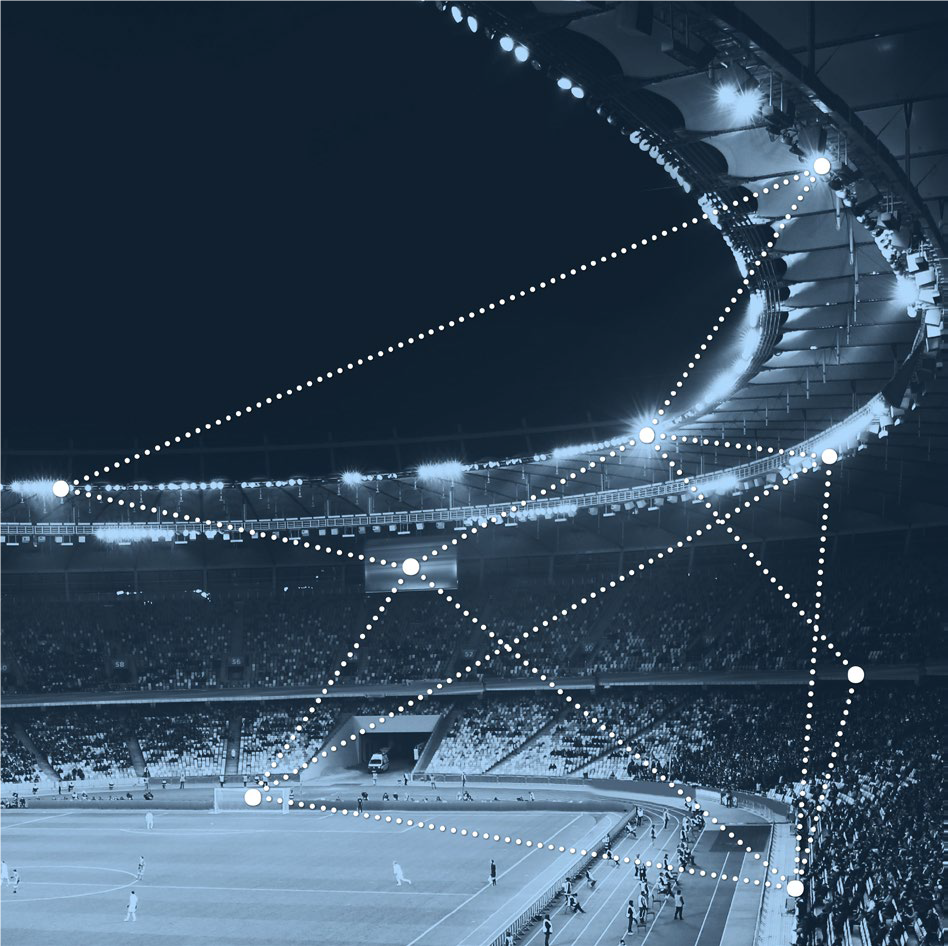
\includegraphics[width=\textwidth]{Bluetooth_Mesh_Stadium_Example.png}
		\caption[Stadion mit Bluetooth-Mesh]{Stadion mit Bluetooth-Mesh \cite{bluetooth_sig_mesh-technology-overviewpdf_2020}}
		\label{fig:BluetoothMeshStadiumExample}
	\end{minipage}
\end{figure}


Die Technologie baut auf den weit verbreitetem BLE-Standard auf, welcher in einer viel zahl von Endgeräten verbaut ist. Ab BLE-Version 4.0 könnten sich die Geräte zu einem Mesh-Netzwerk verbinden. Im Anschluss wird der Netzaufbau kurz erklärt und der Leser mit dem Funktionsprinzip des Mesh-Stacks vertraut gemacht.

Das Einbinden neuer Teilnehmer findet über den Provisioning-Prozess statt. Die Rolle des Provisioners kann ein Smartphone, Laptop oder ein berechtigter Mesh-Teilnehmer übernehmen. Ähnlich wie beim anmelden bei einem WLAN-Netzwerk teilt der Provisioner dem neuen Teilnehmer die Zugangsdaten (Netzwerkschlüssel, etc.) mit. Abschliessend beginnt das neue Gerät im Netzwerk als Node zu operieren. \\  


Bluetooth-Mesh basiert auf dem Managed-Flooding Prinzip. Einfach erklärt wiederholen alle Nodes, abhängig von verschiedenen Bedingungen, jede empfangende Nachricht (Relaying). Somit gelangen die Daten über Zwischenstationen (Hops) zum Ziel. Nachrichten welche nicht für den einzelnen Node relevant sind oder bereits verarbeitet wurden werden verworfen. \\

Um die Funktion von Nodes (Lichtschalter, Lampe, Temperatursensor, etc.) zu unterscheiden, werden sogenannte Models definiert. Jedes Model spezifiziert Zustände (Licht EIN / Licht AUS), welche als States bezeichnet werden. Weiterhin sind Models in drei Kategorien eingeteilt: Server-, Client- und Control-Models. Diese Einteilung schreibt vor ob die Zustände des Nodes zur Veränderung Angeboten werden (Server-Model z.B. Lampe), Zustände verändert werden (Client-Model z.B. Schalter) oder beides möglich ist (Control-Model z.B. Pumpe). Mithilfe dieser Normen lassen sich Geräte von unterschiedlichen Hersteller vereinen, sofern keine Hersteller spezifischen Models verwendet wurden. 

\begin{figure} [H]
	\centering
	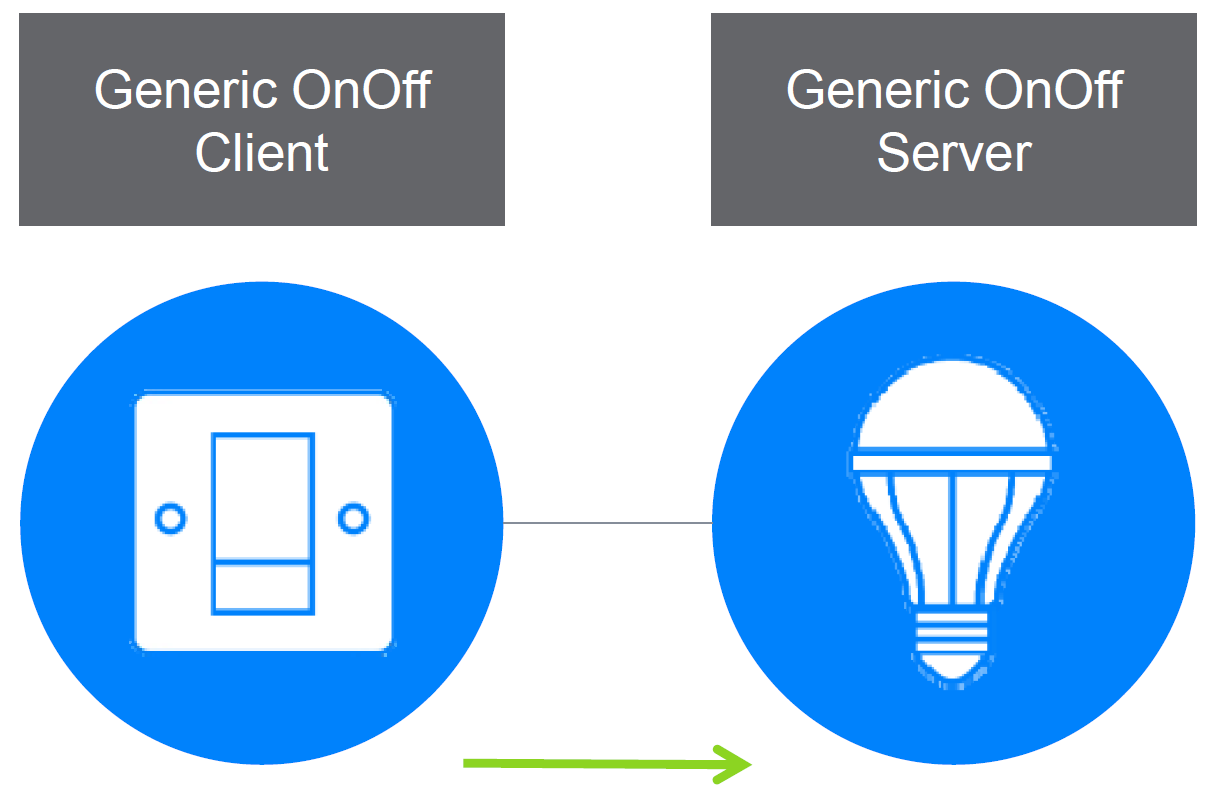
\includegraphics[width=0.6\textwidth]{Bluetooth_Mesh_Client_Server_Prinzip.PNG}
	\caption{Client - Server Prinzip Bluetooth Mesh \cite{bluetooth_sig_mesh-technology-overviewpdf_2020}} 
	\label{fig:BTMeshClientServerPrinzip}
\end{figure}


Zur Identifizierung im Netzwerk besitzt jeder Node eine Unicast-Address (einzigartige Adresse). Um mehrere Nodes zu einer Gruppe zusammenzufassen, werden Group-Addresses vergeben. Die Beziehungen zwischen Nodes werden durch Publishen (Veröffentlichen) oder Subscriben (Abonnieren) auf Adressen geregelt. Im Anwendungsfall Publisht der Client (Schalter) an die Adresse auf welche einer oder mehrere Server (Lampe/Lampen) Subscriben. Wie in Abbildung \ref{fig:BTMeshPublishSubscribePrinzip} ist das Unterscheiden von Bereichen mittels Gruppen möglich. Ein Node kann gleichzeitig an mehrere Adressen Publishen und Subscriben, was zu beliebig komplexen Aufbauten führt. 


\begin{figure} [H]
	\centering
	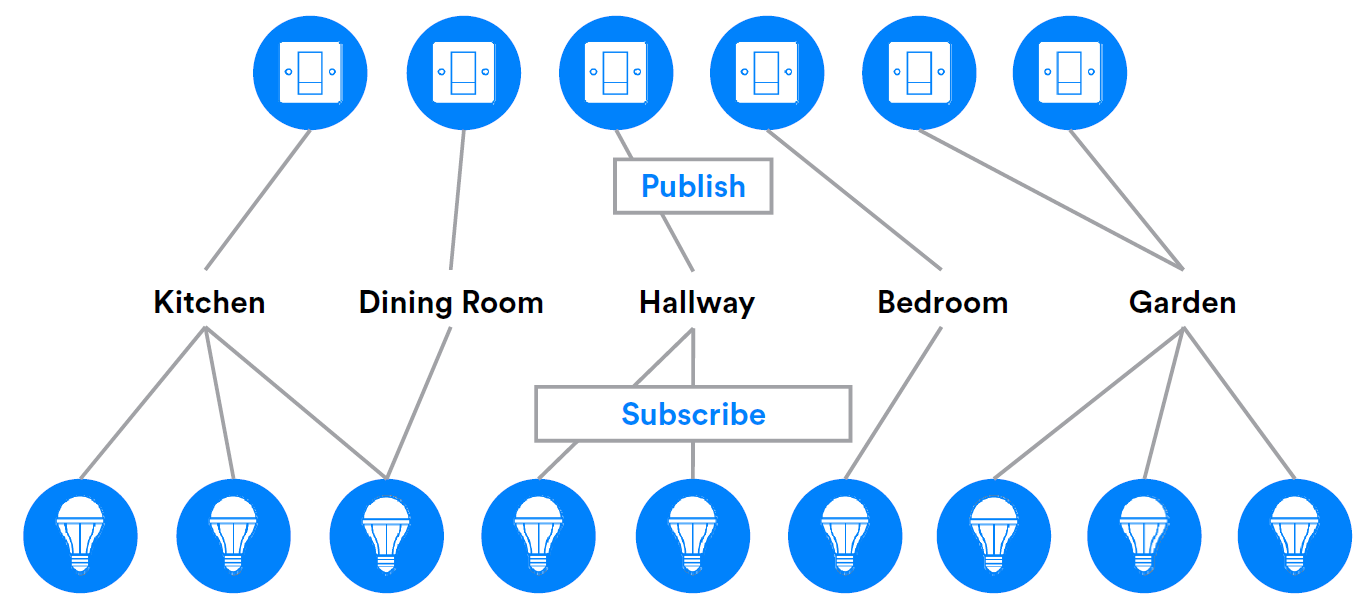
\includegraphics[width=1.0\textwidth]{Bluetooth_Mesh_Publish_Subscribe_Prinzip.PNG}
	\caption{Publish - Subscribe Prinzip Bluetooth Mesh \cite{bluetooth_sig_mesh-technology-overviewpdf_2020}} 
	\label{fig:BTMeshPublishSubscribePrinzip}
\end{figure}









\pagebreak

\clearpage
\section{Technische Grundlagen Bluetooth Mesh}\label{sec:TechnischeGrundlagenBluetoothMesh}

\subsection{Netzaufbau und Topologie}\label{sec:NetzaufbauundTopologie}




\todo[inline]{Welchen Aufbau? Welche Art von Mesh? Welche Nodetypen gibt es? Welche typischen Eigenschaften besitzt das Protokoll?}

\subsection{Bluetooth Mesh Protokoll Stack}\label{sec:ZigbeeProtokollStack}
\todo[inline]{Erläuterung des Protokoll Stacks. Möglichst viel Grafiken und nur so viel als nötig Prosa.}

\subsection{Bluetooth Mesh Software Development Kit}\label{sec:ZigbeeSoftwareDevelopmentKit}
\todo[inline]{Eingesetzte SDK und deren Aufbau beschreiben. Allenfalls die wichtigsten API Funktionen genauer erläutern.}



\pagebreak

\clearpage
\section{Umsetzung Benchmark}\label{sec:BTMeshUmsetzungBenchmark}

Die Umsetzung des Benchmarks, wurde gemäss den Anforderungen des Benchamrk-Konzepts (siehe Abschnitt \ref{sec:BenchmarkKonzeptMeshNetzwerke}) umgesetzt. Zudem wurden die Schnittstellen gemäss dem Software Konzept (siehe Abschnitt \ref{sec:Soft-undFirmware}) an die Shared-Library eingebaut. Im Anschluss wird auf die Umsetzung mittels der SDKs eingegangen, sowie die einzelnen Module dazu Beschrieben. 

\subsection{nRF Connect SDK}\label{subsec:BluetoothMeshUmsetzungnRFConnectSDK} 

Das aufsetzen der nRF Connect SDK, sowie das Installieren der IDE ist online\footnotemark\ Dokumentiert. Mithilfe von Beispielen\footnotemark\ und der Bluetooth-Mesh-API\footnotemark\ wurde die Umsetzung bewerkstelligt. Dabei gliedert sich das Programm in zwei Module welche Nachfolgend beschrieben werden.

\footnotetext{\url{https://developer.nordicsemi.com/nRF_Connect_SDK/doc/latest/nrf/getting_started.html}} 

\footnotetext{\url{https://developer.nordicsemi.com/nRF_Connect_SDK/doc/latest/nrf/samples.html}} 

\footnotetext{\url{https://developer.nordicsemi.com/nRF_Connect_SDK/doc/latest/zephyr/reference/bluetooth/mesh.html}} 

\subsubsection{Stack Initialisierung und Konfiguration}\label{subsubsec:BluetoothMeshUmsetzungnRFConnectSDKInitandConfig} 

Das Modul \textit{bm\_blemesh.c}\footnotemark\ dient zur Initialisierung des Stacks. Dazu wird die Funktion \linebreak\textit{bm\_blemesh\_enable()} aufgerufen. Diese führt die notwendigen Schritte aus um den Mesh-Stack hochzufahren. Nach erfolgreicher Initialisierung wird mit dem Provisioning weitergefahren. \\


\footnotetext{\url{https://github.com/Rouben94/P6_Software/blob/master/Bluetooth/Zephyr_Mesh/src/bm_blemesh.c}}


\paragraph{Self Provisioning}

Um ein vollautomatischen Testablauf zu gewährleisten, wurden die Sicherheitsschlüssel direkt im Code vorgegeben. Mittels der eigens dafür vorgesehenen API \textit{bt\_mesh\_provision} kann sich der Teilnehmer selbst ins Netzwerk einbinden. Dies ist nur zu Testzwecken empfohlen. Die Einbindung der Teilnehmer ins Netz erfolgt somit zuverlässig und unkompliziert.\\

\paragraph{Self Configuring}

Nach der erfolgreichen Einbindung ins Netz, beginnt der Node mit seiner Konfiguration. Ob es sich dabei um einen Client oder Server handelt muss zur Laufzeit bereits bekannt sein. Dies wurde zum Zeitpunkt der Kompilierung mittels der \textit{bm\_config.h} Datei festgelegt. Um Testnachrichten zu senden oder zu Empfangen wurde das Generic ON/OFF Server- resp. Client-Model eingesetzt. Des weiteren werden die Models initialisiert, an den Applikations-Key gebunden und die Publish- oder Subsrcibe-Adressen auf die jeweilige Group-Address konfiguriert. Diese Werte sind entweder aus der vorhergehenden Konfiguration bekannt oder wurden fest vorgegeben. Der Teilnehmer ist nun bereit Nachrichten zu Senden oder zu Empfangen. 


 
 

\subsubsection{Model Handler}\label{subsubsec:BluetoothMeshUmsetzungnRFConnectSDKModelHandler}

Das Modul \textit{bm\_blemesh\_model\_handler.c}\footnotemark\ beherbergt alle notwendigen Model-Handler, welche zum Senden oder Empfangen von Nachrichten aufgerufen werden. In den jeweiligen Handlern soll ein Log-Eintrag mit den entsprechenden Informationen aufgefüllt werden. 


\footnotetext{\url{https://github.com/Rouben94/P6_Software/blob/master/Bluetooth/Zephyr_Mesh/src/bm_blemesh_model_handler.c}}


\paragraph{Message Sending}

Um eine Nachricht zu senden wird eine universelle Schnittstelle der Shared-Library zur Verfügung gestellt. Diese kann mittels dem Aufrufen der Funktion \textit{bm\_send\_message(}) eine Nachricht versenden. Anschliessend wird der entsprechende Handler des Generic ON/OFF Clients benachrichtigt. Dieser wechselt den Zustand des grünen RGB-LEDs, speichert eine Log-Eintrag und schickt die Nachricht ab. Dieser wird, gemäss der Konfiguration des Nodes, acknowledged oder unacknowledged  und mit der zusätzlichen anzahl Bytes gesendet. 

\paragraph{Message Receiving} 

Sobald eine Nachricht vom Stack empfangen wurde, wird der Handler des Generic ON/OFF Servers benachrichtigt. Im Handler-Kontext sind viele notwendige Informationen für das Log bereits enthalten. Das erfassen des Zeitstempels und abfragen der Nachrichtenlänge wird über externe Funktionsaufrufe und Hilfsvariablen bewerkstelligt. Schlussendlich wird die blaue RGB-LED geschaltet, welches den erfolgreichen Empfang einer Nachricht anzeigt. 


\subsection{Benchmark und Stack Parameter}\label{subsec:BT_MESHBenchmarkundStackParameter}

Die Tabelle \ref{tab:BT_MESHBenchmarkundStackParameter} soll einen Überblick der verwendeten Paramter des Stacks geben. 



\begin{table}[h]
	\centering
	\begin{adjustbox}{width=1\textwidth}
		\begin{tabular}{|l|l|l|} 
			\hline
			Stack Init Time & 10000 ms & \begin{tabular}[c]{@{}l@{}}Zeit die benötigt wird um den Stack für den Benchmark\\zu initialisieren. \end{tabular} \\ 
			\hline
			\multicolumn{1}{l}{} & \multicolumn{1}{l}{} & \multicolumn{1}{l}{} \\ 
			\hline
			Node Type & Relay-Node & Alle Nodes werden als Relay-Nodes konfiguriert \\ 
			\hline
			Default~Group ID & 0xC000 & \begin{tabular}[c]{@{}l@{}}Zu diesem Wert wird der Index für die\textcolor[rgb]{0.502,0,0}{ }zugewiesene Gruppe\\addiert um damit die Gruppenzugehörigkeit festzulegen.\end{tabular} \\ 
			\hline
		\end{tabular}
	\end{adjustbox}
	\caption{Bluetooth Mesh Benchmark und Stack Parameter}
	\label{tab:BT_MESHBenchmarkundStackParameter}
\end{table}

Ein detailierte Konfiguration des Zephyr Kconfig kann übder den Source-Code\footnotemark\ abgefragt werden. 

\footnotetext{\url{https://github.com/Rouben94/P6_Software/blob/master/Bluetooth/Zephyr_Mesh/prj.conf}}


\subsection{nRF SDK for Mesh}\label{subsec:BluetoothMeshUmsetzungnRFSDKMesh} 

Die Umsetzung mittels der \textit{nRF SDK for Mesh} wurde noch nicht vollumfänglich abgeschlossen. Es liegen zurzeit Probleme beim Zugriff auf den Flash-Treiber vor, welche noch zu beheben sind. Die Umsetzung des Benchmarks wurde jedoch abgeschlossen und es können Nachrichten versandt sowie empfangen werden. Das Loggen der Informationen funktioniert ebenfalls. \\

Das aufsetzen der \textit{nRF SDK for Mesh}, sowie das Installieren der IDE ist online\footnotemark\ Dokumentiert. Mithilfe von Beispielen\footnotemark\ und der Bluetooth-Mesh-API\footnotemark\ wurde die Umsetzung bewerkstelligt. Dabei gliedert sich das Programm in zwei Module, welche Nachfolgend beschrieben werden.\\

Die Umsetzung wurde ähnlich realisiert wie mit der \textit{nRF Connect SDK}. Im Anschluss sind die Unterschiede aufgezeigt. 



\footnotetext{\url{https://infocenter.nordicsemi.com/topic/com.nordic.infocenter.meshsdk.v4.2.0/md_doc_getting_started_getting_started.html}} 

\footnotetext{\url{https://infocenter.nordicsemi.com/topic/com.nordic.infocenter.meshsdk.v4.2.0/md_examples_light_switch_README.html}} 

\footnotetext{\url{https://infocenter.nordicsemi.com/topic/com.nordic.infocenter.meshsdk.v4.2.0/modules.html}} 

\subsubsection{Stack Initialisierung und Konfiguration}\label{subsubsec:BluetoothMeshUmsetzungnRFSDKInitandConfig} 

Das Modul \textit{bm\_ble\_mesh.c}\footnotemark\ sowie das Modul \textit{bm\_mesh\_stack.c}\footnotemark\ dienen zur Initialisierung des Stacks. Dazu wird die Funktion \textit{bm\_blemesh\_init()} aufgerufen. Diese führt die notwendigen Schritte aus um den Mesh-Stack hochzufahren. Nach erfolgreicher Initialisierung wird mit dem Provisioning weitergefahren. \\


\footnotetext{\url{https://github.com/Rouben94/P6_Software/blob/master/Bluetooth/nRF_SDK_Mesh/src/bm_ble_mesh.c}}

\footnotetext{\url{https://github.com/Rouben94/P6_Software/blob/master/Bluetooth/nRF_SDK_Mesh/src/bm_mesh_stack.c}}

\paragraph{Self Provisioning and Configuring}

Das Self Provisioning sowie das Self Configuring werden bei der \textit{nRF SDK for Mesh} mittels dem Device-State-Manager durchgeführt. Dieser verwaltet alle notwendigen Keys sowie Address-Listen, welche zur Konfiguration gebraucht werden. Durch analysieren des Config-Server-Models, welches normalerweise die Konfiguration des Nodes vornimmt, wurde der notwendige Ablauf zur Konfiguration rekonstruiert. 

\subsubsection{Model Handler}\label{subsubsec:BluetoothMeshUmsetzungnRFSDKModelHandler}

Die Model-Handler sind im Modul \textit{bm\_ble\_mesh.c}\footnotemark\ integriert. Das Empfangen und Senden von Nachrichten wird ähnlich wie bei der \textit{nRF Connect SDK} abgehandelt. 

\pagebreak


%%Part 2 Thread

\vspace*{4cm}
\part{Thread}\label{part:Thread}
Robin Bobst
\vspace*{\fill}
\clearpage

\section{Einleitung}\label{sec:EinleitungThread}
Thread ist ein auf IPv6 basiertes Netzwerkprotokoll, das speziell für Internet of Things (IoT) Anwendungen entwickelt wurde. Die einzelnen Teilnehmer im Netzwerk verbinden sich zu einem Mesh-Netzwerk. Wie in der Abbildung \ref{fig:ThreadProtokollLayer} ersichtlich verwendet Thread für eine effiziente Kommunikation mit IPv6-Paketen das Kommunikationsprotokoll 6LoWPAN (IPv6 over Low Power Personal Area Network). 6LoWPAN wendet ein Header-Kompressionsverfahren an, welches es ermöglicht die IPv6-Pakete über den Standard IEEE-802.15.4 zu übermitteln. Dank diesem Standard ist es machbar, die mit Thread entwickelten Geräte so energieeffizient zu gestalten, dass ein Batteriebetrieb realisierbar ist. In der Tabelle \ref{table:MerkmaleThread} sind die wichtigsten Merkmale von Thread aufgelistet. Im Juli 2014 wurde die Thread Working Group ins Leben gerufen, bei der folgende Firmen Bestandteil der Gruppe sind: Nest Labs, Samsung, ARRM Holdings, Qualcom, NXP Semiconductors, Silicon Labs, Big Ass Solutions, Somfy, OSRAM Tyco International und Yale. Ab August 2018 Apple trat auch Apple der Arbeitsgruppe bei, um das Prokoll populär zu machen. \cite[Kapitel 1]{thread_group_inc_thread_2017} \\

\begin{figure}[H]
	\centering
	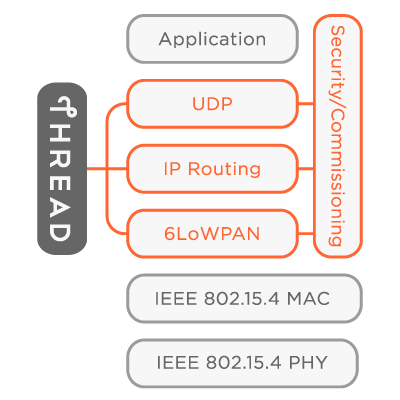
\includegraphics[width=0.5\textwidth]{threadlayerprotocols.png}
	\caption{Thread Protokoll Layer \cite{erickson_picture_2019}}
	\label{fig:ThreadProtokollLayer}
\end{figure}

\begin{table}[H]
	\centering
	\begin{adjustbox}{width=1\textwidth}
	\begin{tabular}{@{}lllll@{}}
		\cmidrule(r){1-2} \cmidrule(l){4-5}
		\multicolumn{2}{|c|}{\textbf{Netzwerk}}                                                              & \multicolumn{1}{l|}{} & \multicolumn{2}{c|}{\textbf{Applikation}}                                                                           \\ \cmidrule(r){1-2} \cmidrule(l){4-5} 
		\multicolumn{1}{|l|}{\textbf{Merkmal}}      & \multicolumn{1}{l|}{\textbf{Beschreibung}}             & \multicolumn{1}{l|}{} & \multicolumn{1}{l|}{\textbf{Merkmal}}                   & \multicolumn{1}{l|}{\textbf{Beschreibung}}                \\ \cmidrule(r){1-2} \cmidrule(l){4-5} 
		\multicolumn{1}{|l|}{IEEE 802.15.4}         & \multicolumn{1}{l|}{Protokoll}                         & \multicolumn{1}{l|}{} & \multicolumn{1}{l|}{IPv6}                               & \multicolumn{1}{l|}{IP-Kommunikation}                     \\ \cmidrule(r){1-2} \cmidrule(l){4-5} 
		\multicolumn{1}{|l|}{MAC Security}          & \multicolumn{1}{l|}{Verschlüsselte Übertragung}        & \multicolumn{1}{l|}{} & \multicolumn{1}{l|}{UDP}                                & \multicolumn{1}{l|}{UDP-Sockets}                          \\ \cmidrule(r){1-2} \cmidrule(l){4-5} 
		\multicolumn{1}{|l|}{6LoWPAN}               & \multicolumn{1}{l|}{Effiziente IPv6 Paket Übertragung} & \multicolumn{1}{l|}{} & \multicolumn{1}{l|}{CoAP}                               & \multicolumn{1}{l|}{Client und Server}                    \\ \cmidrule(r){1-2} \cmidrule(l){4-5} 
		\multicolumn{1}{|l|}{Mesh Routing}          & \multicolumn{1}{l|}{Many-to-many Kommunikation}        & \multicolumn{1}{l|}{} & \multicolumn{1}{l|}{DHCPv6}                             & \multicolumn{1}{l|}{Client und Server}                    \\ \cmidrule(r){1-2} \cmidrule(l){4-5} 
		&                                                        &                       &                                                         &                                                           \\ \cmidrule(r){1-2} \cmidrule(l){4-5} 
		\multicolumn{2}{|c|}{\textbf{Boarder Router}}                                                        & \multicolumn{1}{l|}{} & \multicolumn{2}{c|}{\textbf{Weitere Merkmale}}                                                                      \\ \cmidrule(r){1-2} \cmidrule(l){4-5} 
		\multicolumn{1}{|l|}{Web - UI}              & \multicolumn{1}{l|}{Für Netzwerk Menagement}           & \multicolumn{1}{l|}{} & \multicolumn{1}{l|}{Periodic parent search}             & \multicolumn{1}{l|}{Endgerät wechselt zu besserem Parent} \\ \cmidrule(r){1-2} \cmidrule(l){4-5} 
		\multicolumn{1}{|l|}{Externer Kommissioner} & \multicolumn{1}{l|}{Externes Gerät für Neuaufnahme}    & \multicolumn{1}{l|}{} & \multicolumn{1}{l|}{Jam Detection}                      & \multicolumn{1}{l|}{Signal Stau verhindern}               \\ \cmidrule(r){1-2} \cmidrule(l){4-5} 
		\multicolumn{1}{|l|}{NAT64}                 & \multicolumn{1}{l|}{Kommunikation mit IPv4}            & \multicolumn{1}{l|}{} & \multicolumn{1}{l|}{Child Supervision}                  & \multicolumn{1}{l|}{Endgerät überprüfen}                  \\ \cmidrule(r){1-2} \cmidrule(l){4-5} 
		\multicolumn{1}{|l|}{wpantund}              & \multicolumn{1}{l|}{Interface Treiber}                 & \multicolumn{1}{l|}{} & \multicolumn{1}{l|}{Inform previous parent on reattach} & \multicolumn{1}{l|}{Endgerät Menagement}                  \\ \cmidrule(r){1-2} \cmidrule(l){4-5} 
	\end{tabular}
	\end{adjustbox}
	\caption{Merkmale Thread \cite{thread_group_what_2020}}
	\label{table:MerkmaleThread}
\end{table}


\pagebreak

\clearpage
\section{Technische Grundlagen Thread}\label{sec:TechnischeGrundlagenThread}

\subsection{Netzaufbau und Topologie}\label{subsec:NetzaufbauundTopologie}
\todo[inline]{Welchen Aufbau? Welche Art von Mesh? Welche Nodetypen gibt es? Welche typischen Eigenschaften besitzt das Protokoll?}
\subsubsection{Node Typen}\label{subsubsec:NodeTypen}
\textbf{Full Thread Device (FTD)}

\underline{Leader:}

\underline{Router:}

\underline{Full End Device:}

\textbf{Minimal Thread Device (MTD)}

\underline{Minimal End Device:}

\underline{Sleepy End Device:}

\subsubsection{IPv6 Adressierung}\label{subsubsec:IPv6Adressierung}

\subsubsection{Netzwerk Aufbau}\label{subsubsec:NetzwerkAufbau}

\subsubsection{Router Auswahl}\label{subsubsec:RouterAuswahl}

\subsection{Application Layer}\label{subsec:CoAP}

\subsection{Thread Protokoll Stack}\label{subsec:ThreadProtokollStack}
\todo[inline]{Erläuterung des Protokoll Stacks. Möglichst viel Grafiken und nur so viel als nötig Prosa.}
\subsubsection{UDP}\label{subsubsec:UDP}
\subsubsection{IP Routing}\label{subsubsec:IPRouting}
\subsubsection{6LoWPAN}\label{subsubsec:6LoWPAN}

\subsection{Link und Physical Layer}\label{subsec:IEE802154}

\subsection{Thread Software Development Kit}\label{subsec:ThreadSoftwareDevelopmentKit}
\todo[inline]{Eingesetzte SDK und deren Aufbau beschreiben. Allenfalls die wichtigsten API Funktionen genauer erläutern.}

\pagebreak

\clearpage
\section{Firmware Benchmark}\label{sec:FirmwareBenchmark}
\todo[inline]{Komplette Beschreibung der Firmware unterteilt in die 3 Nodetypen. Besonderheiten herausstreichen und allfällige Schwierigkeiten aufzeigen.}


\subsection{Benchmark Master}\label{sec:BenchmarkMasterThread}


\subsection{Benchmark Server}\label{sec:BenchmarkServerThread}


\subsection{Benchmark Client}\label{sec:BenchmarkClientThread}
\pagebreak



%%Part 3 Zigbee

\vspace*{4cm}
\part{Zigbee}\label{part:Zigbee}
Autor: Cyrill Horath
\vspace*{\fill}
\clearpage

\section{Einleitung}\label{sec:EinleitungZigbee}
In diesem Teil der Arbeit werden die Eigenschaften und Besonderheiten des Zigbee Mesh Stack erläutert und es wird auf die Umsetzung des Benchmarks auf Stack Ebene eingegangen. Dieser Teil soll als eigenständiger Teil betrachtet werden in dem ausschliesslich Zigbee behandelt wird.

Zigbee ist ein auf dem IEEE 802.15.4 Standard aufbauendes drahtloses Low Power Mesh Netzwerk. Es nutzt das vom IEEE 802.15.4 Standard definierte ISM-Funkfrequenzband 2.4GHz plus weitere Sub-GHz Bänder je nach Region.
Die im Jahre 2002 gegründete Zigbee Allianz spezifiziert den Protokoll Standard und gibt seit da an laufend Neuerungen und Updates heraus.
Im Zuge der Verbreitung von Technologien in der Heim Automatisierung erhielt auch Zigbee immer mehr Aufmerksamkeit und wuchs bis heute zum wohl am weitesten verbreiteten Mesh Netzwerk Protokoll in diesen Gebiet heran. Besonders in Systemen für die Steuerung von Beleuchtungen wie zum Beispiel Phillips Hue und Ikea Tradfri kommt Zigbee verbreitet zum Einsatz.

Die Spezifikationen innerhalb des Zigbee Protokollstacks sind weitreichend. Von der MAC Ebene über die Netzwerkschicht bis hin zur Applikationsebene gibt es klare Vorgaben wie ein Zigbee Produkt aufgebaut sein soll.
Mit der \textit{Zigbee Cluster Library} werden sogar spezifische Anwendungen vordefiniert wie beispielsweise die Steuerung eine Lichtquelle mit Dimmfunktion.
Diese Spezifikationen ermöglichen die Interoperabilität von Systemen mit der gleichen Funktion jedoch von unterschiedlichen Herstellern.





\pagebreak

\clearpage
\section{Technische Grundlagen Zigbee}\label{sec:TechnischeGrundlagenZigbee}

\subsection{Netzaufbau und Topologie}\label{subsec:NetzaufbauundTopologie}
\todo[inline]{Welchen Aufbau? Welche Art von Mesh? Welche Nodetypen gibt es? Welche typischen Eigenschaften besitzt das Protokoll?}


Zigbee ist nicht gleich Zigbee. Obwohl Zigbee von zentraler Stelle, der Zigbee Alliance, spezifiziert wurde gibt es verschiedene Arten davon. In den Spezifikationen wird zwischen zwei sogenannten Stackprofilen \textit{ZigBee} und \textit{ZigBee PRO} unterschieden.
Während \textit{ZigBee}-Netzwerke eine Baumstruktur haben und der Koordinator dabei einen Single-Point-of-Failure bildet, bieten \textit{ZigBee PRO}-Netzwerke geroutete Mesh Funktionalitäten mit Routing Tabellen und Wegentdeckung. Der Koordinator bildet dabei nicht länger einen Single-Point-of-Failure da sich das Routing dynamisch anpassen kann.
Die Abbildung \ref{fig:NetzwerktopologienZigbee} zeigt die Unterschiede von einem Baumnetzwerk im Stackprofil \textit{ZigBee} links und einem Meshnetzwerk im Stackprofil \textit{ZigBee PRO} rechts.
In der vorliegenden Arbeit wurde das \textit{ZigBee PRO} Stackprofil verwendet womit vollwertige Meshnetzwerke möglich sind.

\begin{figure}[h]
	\centering
	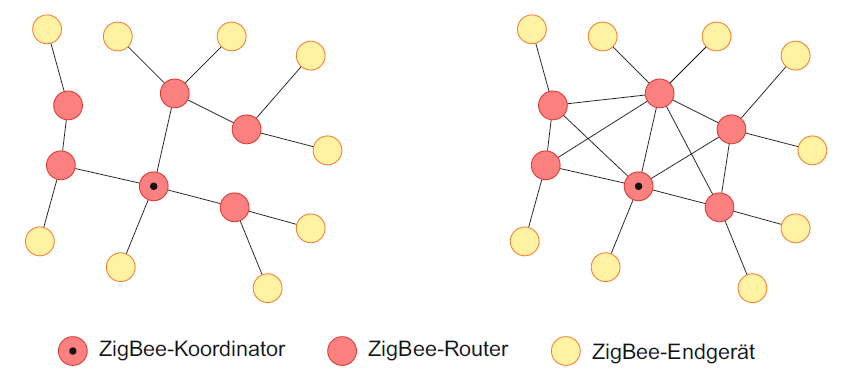
\includegraphics[width=0.8\textwidth]{Zigbee_Netztopologie.png}
	\caption{Zigbee Baum- und Meshnetzwerke \cite[S.~221]{markus_krause_rainer_konrad_zigbee_2014}}	\label{fig:NetzwerktopologienZigbee}
\end{figure}

Wie in der Abbildung \ref{fig:NetzwerktopologienZigbee} bereits angedeutet, kann innerhalb eines Zigbee Meshnetzwerkes zwischen 3 Nodetypen unterschieden werden. Diese besitzen unterschiedliche Aufgaben und Eigenschaften.

\paragraph{Zigbee Koordinator}\label{par:ZigbeeKoordinator}
Als zentrale Einheit übernimmt der \textit{Zigbee Koordinator} Aufgaben wie den Start und die Verwaltung eines PAN (Personal Area Network) inkl. der Definition der wichtigsten Parameter wie der PAN-ID, der Sicherheitsschlüssel sowie die Wahl des IEEE Channels.
In einem Zigbee-Netzwerk gibt es genau ein Gerät das die Rolle des \textit{Zigbee Koordinators} übernimmt. Wenn dieses Gerät das Netzwerk verlässt oder kurzzeitig ausser Betrieb ist, kann das Netzwerk trotzdem weiter bestehen und funktioniert normal weiter.
Jeder \textit{Zigbee-Koordinator} hat gleichzeitig auch die Rolle eines \textit{Zigbee-Router}.

\paragraph{Zigbee Router}\label{par:ZigbeeRouter}
\textit{Zigbee-Router} bilden das eigentliche Meshnetzwerk. Sie übernehmen die Aufgabe des Routings was die Wegentdeckung sowie Weiterleitung von Paketen beinhaltet. Jeder \textit{Zigbee-Router} führt eine Routing-Table welche fortlaufend aktualisiert wird.

\paragraph{Zigbee End-Device}\label{par:ZigbeeEndDevice}
Die einfachste Rolle ist jene des \textit{Zigbee End-Devices}. Sie stehen in einer Parent-Child Beziehung mit einem \textit{Zigbee-Router}.
Diese Kommunikation findet entweder periodisch oder ausgelöst durch einen Userinput statt.
Ankommende Pakete werden jeweils vom Parent-Node gespeichert bis das  \textit{Zigbee End-Devices} diese abruft.
\textit{Zigbee End-Devices} besitzen ausserdem keine Routing Funktionen und gelten deshalb als sehr energiesparend.
Ausgeführt als Sleepy-End-Device können CPU und RAM des entsprechenden Nodes ganz oder teilweise heruntergefahren werden und durch periodische Interrupts geweckt werden.
Dadurch können sehr lange Batteriestandzeiten erreicht werden. \cite{markus_krause_rainer_konrad_zigbee_2014}


\subsection{Zigbee Protokoll Stack}\label{subsec:ZigbeeProtokollStack}
\todo[inline]{Erläuterung des Protokoll Stacks. Möglichst viel Grafiken und nur so viel als nötig Prosa.}

Die Architektur des Zigbee Stacks besteht aus vier Layern, dem Physical layer (PHY), dem MAC layer, dem Network layer (NWK) und dem Application layer (APL).
Abbildung \ref{fig:ArchitekturdesZigbeeProtokollStacks} zeigt den Aufbau des Protokoll Stacks im Detail.
Jede der Schichten ist mit bestimmten Aufgaben betraut und stellt der darüber liegenden Schicht Daten und Dienste bereit.
Nachfolgend wird auf die vier Schichten des Zigbee Stacks eingegangen und deren Funktion und Funktionsweise kurz erläutert.

\begin{figure}[h]
	\centering
	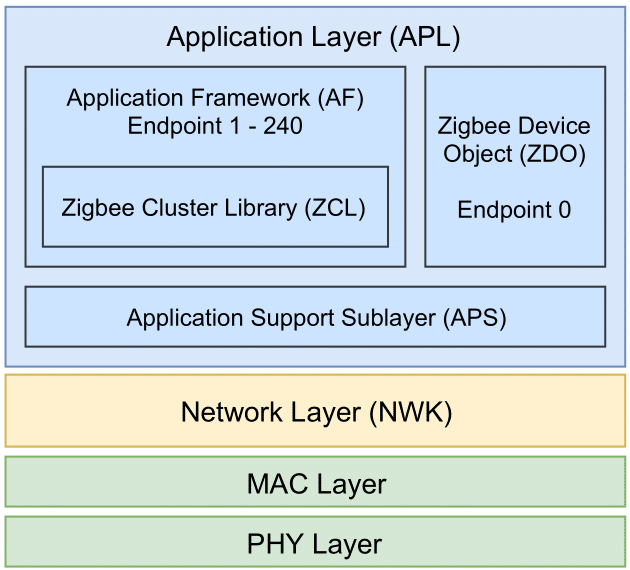
\includegraphics[width=0.7\textwidth]{Zigbee_Architektur.png}
	\caption{Architektur des Zigbee Protokoll Stacks}
	\label{fig:ArchitekturdesZigbeeProtokollStacks}
\end{figure}

\subsubsection{MAC und PHY Layer}\label{subsubsec:MACundPHYLayer}
MAC und PHY Layer werden im Zigbee Protokoll Stack gebildet durch den IEEE 802.15.4 Standard für \textit{Wireless Personal Area Networks (WPAN)}.
Während beispielsweise Wifi oder Bluetooth, welche auf dem selben 2.4 GHz ISM-Funkfrequenzband betrieben werden können, für hohe Datenübertragungsraten konzipiert wurden, ist dieser Standard für kleinere Datenmengen optimiert.
Durch die Vermeidung von unnötigen Steuerinformationen, kann der IEEE 802.15.4 Standard auf einfachster Hardware realisiert und mit kleinstem Energieaufwand betrieben werden.
Ideal also für sogenannte \textit{Wireless Sensor Networks (WSN)} wie beispielsweise Zigbee. \cite{markus_krause_rainer_konrad_ieee_2014}


\subsubsection{Network Layer}\label{subsubsec:Network Layer}
Der Network Layer ist im Zigbee Stack verantwortlich für den Aufbau sowie das Management der Netzwerkfunktionen und das Routing innerhalb dieses Netzwerkes.

\paragraph{Netzaufbau und Adressierung}\label{par:ZigbeeNetzaufbauundAdressierung}
Wie unter \ref{par:ZigbeeKoordinator} bereits erwähnt ist der Koordinator verantwortlich für den Aufbau des Zigbee Netzwerks und der Wahl von entsprechend geeigneten Parametern wie beispielsweise einer 16-Bit PAN-ID oder eines möglichst störungsfreien Funkkanals.
Beim Beitritt eines neuen Funkmoduls wird diesem vom Koordinator eine im Netzwerk einmalige 16-Bit \textit{Short-Address} zugewiesen.
Anhand dieser kann das Funkmodul nun im Netzwerk adressiert werden und es selbst kann damit Routing Funktionen war nehmen.
Die im MAC Layer definierte 64-Bit MAC Adresse kann ebenfalls vollwertig für die Adressierung verwendet werden wobei diese schliesslich in die \textit{Short-Address} übersetzt wird.


\paragraph{Routing}\label{par:Zigbee Routing}
Das Routing geschieht innerhalb von Zigbee Mesh Netzwerken mit dem \textit{ZigBee PRO}-Stackprofil mittels Routingtabellen die jeder Router erstellt und nach führt wenn es Änderungen gibt. In dieser ist die \textit{Short-Address} des Ziels sowie jene des nächsten Hops hinterlegt.
Enthält die Routingtabelle veraltete Einträge oder sind für das entsprechende Ziel noch gar keine Informationen vorhanden, muss ein \textit{Route Discovery} durchgeführt werden.
Hierbei handelt es sich um eine Broadcast Nachricht welche an alle Router gesendet wird. Diese empfangen die Nachricht und leiten sie wiederum als Broadcast an alle Router in Reichweite weiter. Dabei werden die Wegkosten jeweils addiert um diese sobald die Nachricht beim Zielnode angekommen ist, dem Absender mitzuteilen.
Jener Weg mit den geringsten totalen Wegkosten wir so ermittelt und kann schliesslich in der Routingtabelle abgelegt werden.


\subsubsection{Application Support Sublayer (APS)}\label{subsubsec:ApplicationSupportSublayer}


\subsubsection{Application Layer}\label{subsubsec:ZigbeeApplicationLayer}

\paragraph{Zigbee Cluster Library (ZCL)}\label{par:ZigbeeClusterLibrary}

\paragraph{Endpunkte}\label{par:ZigbeeEndpunkte}


\subsubsection{Sicherheit}\label{subsucsec:ZigbeeSicherheit}



\subsection{Zigbee Software Development Kit}\label{subsec:ZigbeeSoftwareDevelopmentKit}
\todo[inline]{Eingesetzte SDK und deren Aufbau beschreiben. Allenfalls die wichtigsten API Funktionen genauer erläutern.}

nRF5 SDK for Thread and Zigbee

ZBOSS stack v3.3.0

Kooperatives Multitasking in ZBOSS

revision 22 of the Zigbee Core Specification.
 
 \begin{figure}[h]
	\centering
	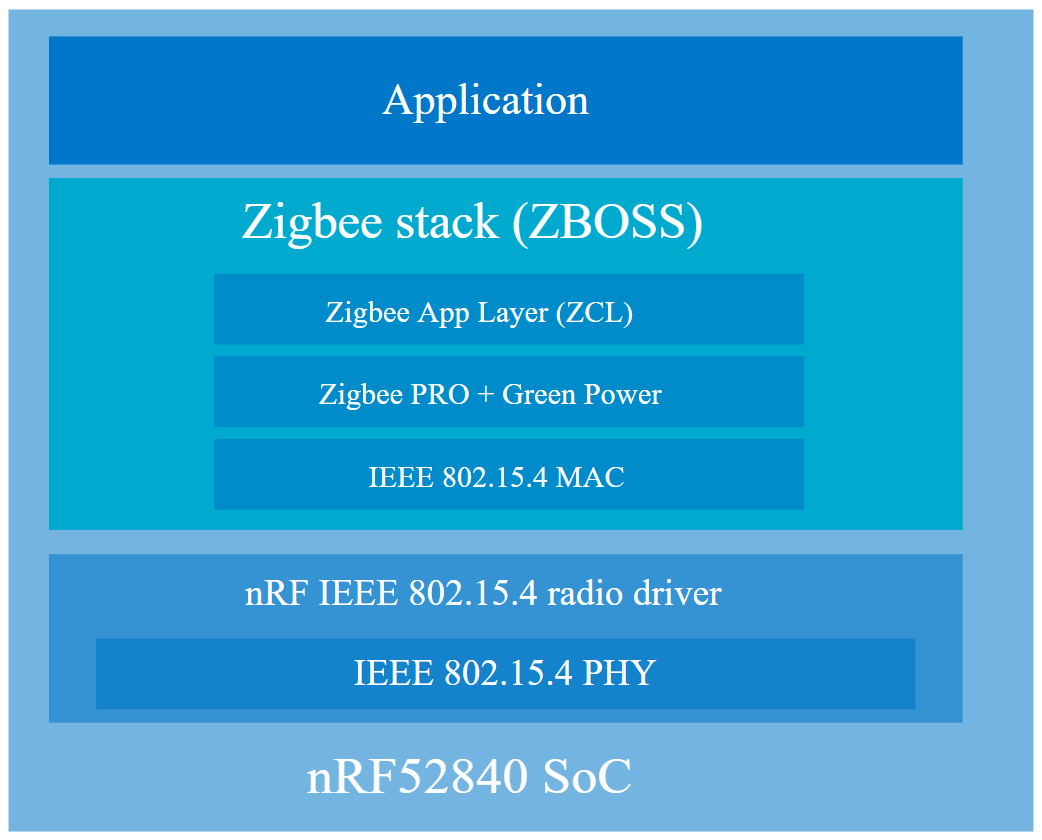
\includegraphics[width=0.6\textwidth]{Zigbee_SDK_Plattform_Design.png}
	\caption{nRF5 SDK for Thread and Zigbee Plattform Design Referenz \cite{nordic_semi_nrf_sdk_for_thread_and_zigbee_2020}}
	\label{fig:ZigbeePlattformDesign}
\end{figure}
 
\pagebreak

\clearpage
\section{Umsetzung Benchmark}\label{sec:UmsetzungBenchmark}
\todo[inline]{Komplette Beschreibung der Firmware unterteilt in die 3 Nodetypen. Besonderheiten herausstreichen und allfällige Schwierigkeiten aufzeigen.}



\subsection{Benchmark Message}\label{subsec:BenchmarkMessage}

\subsection{Zigbee Stack Implementation}\label{subsec:ZigbeeStackImplementation}

\subsubsection{Funkkanal Wahl im 2.4GHz ISM Band}\label{subsubsec:FunkkanalWahlim2.4GHzISMBand}

\begin{figure}[h]
	\centering
	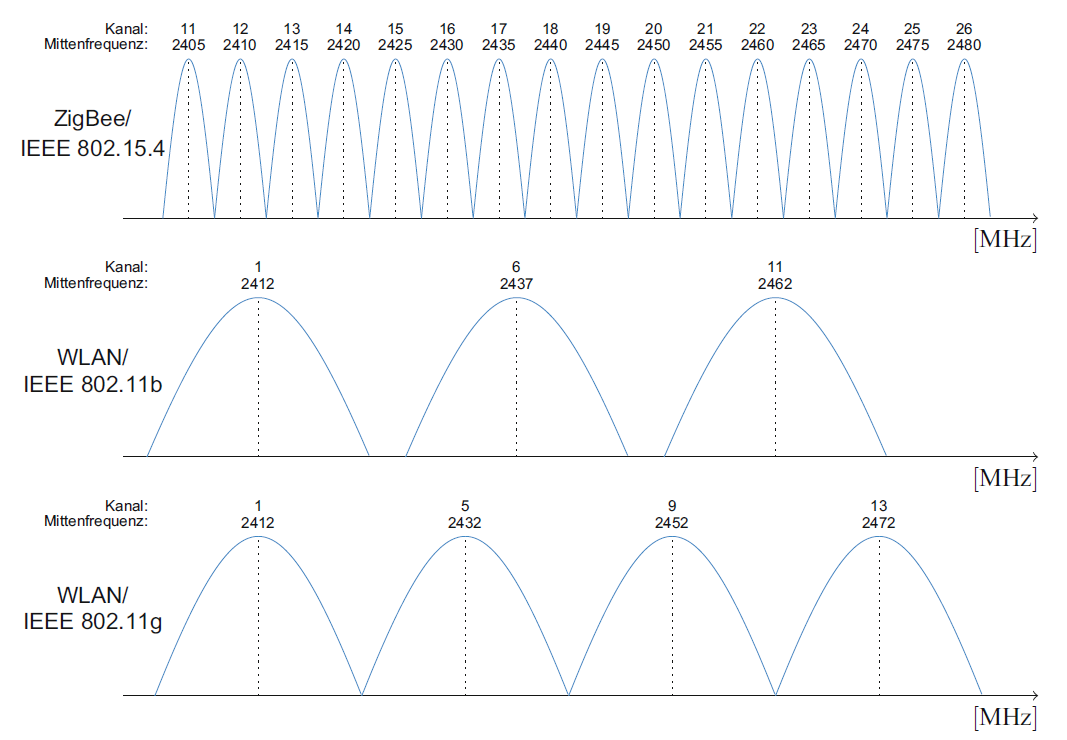
\includegraphics[width=\textwidth]{Funkkanaele_Konkurrenz_IEEE.png}
	\caption{Konkurrenz IEEE und WLAN Funkkanäle \cite{markus_krause_rainer_konrad_drahtlose_2014}}
	\label{fig:KonkurrenzIEEEundWLANFunkkanäle}
\end{figure}

\subsubsection{ZCL Level Cluster}\label{subsubsec:ZCLLevelCluster}

\subsubsection{Endpoint Handler}\label{subsubsec:EndpointHandler}

\subsubsection{APS Header}\label{subsubsec:Header}

\subsubsection{Adressierung}\label{subsubsec:Adressierung}


\pagebreak
%


\clearpage
%%---BIBLIOGRAPHY------------------------------------------------------------------------
{\sloppypar
\printbibliography[heading=bibintoc]
\label{sec:lit}
%\selectlanguage{ngerman}				%ngerman or english
%\printbibliography
}

%%---List of Figures------------------------------------------------------------------------
\listoffigures

%%---APPENDIX----------------------------------------------------------------------------
\begin{appendix} 

\addcontentsline{toc}{section}{Anhang}


%**********************Aufgabenstellung***************************
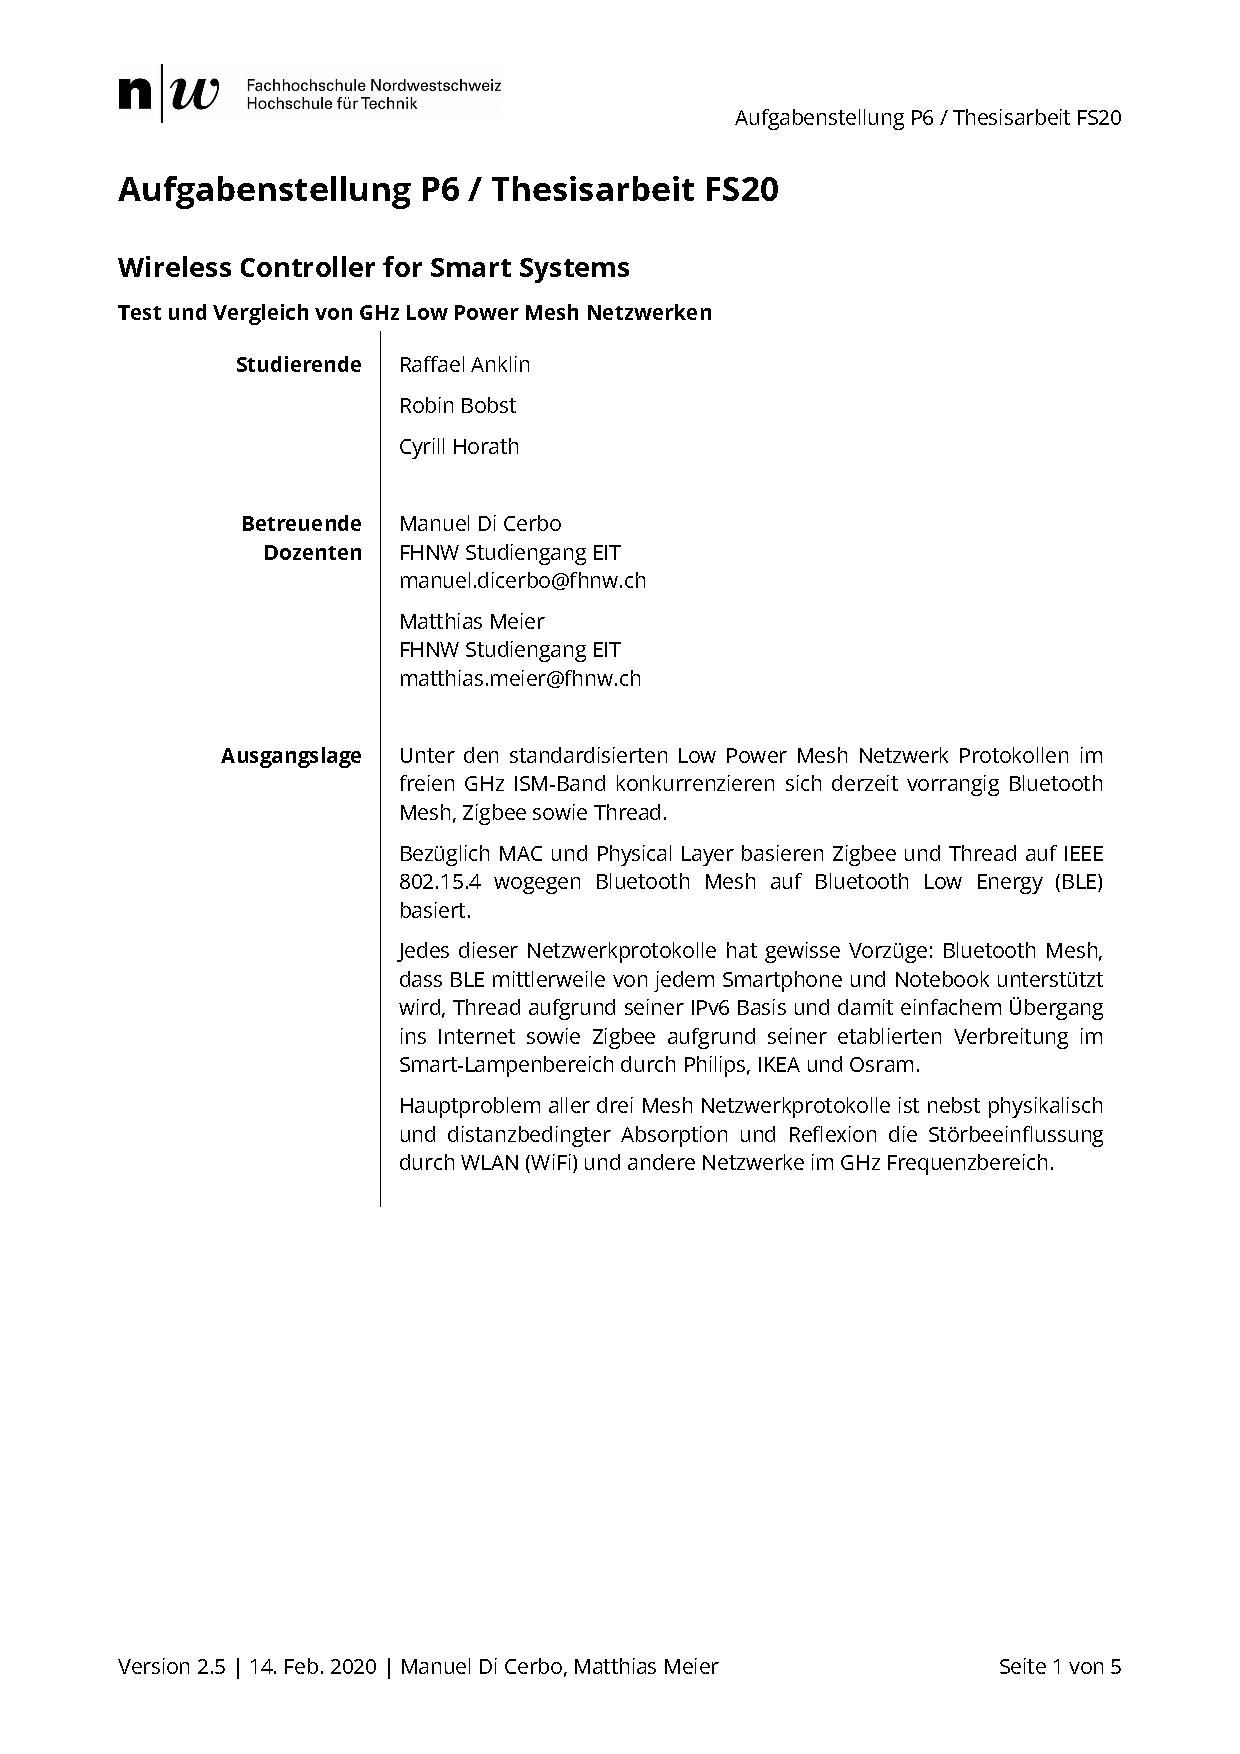
\includepdf[pages={1}, nup=1x1, landscape=false, scale=0.9 ,offset=0 -45, pagecommand={\section{Aufgabenstellung}\label{app:Aufgabenstellung}\thispagestyle{myheadings}}]{appendix/P6_Aufgabenstellung_Wireless_Controller_for_Smart_Systems.pdf}

\includepdf[pages={2-5}, nup=1x1, landscape=false, scale=0.9 ,offset=0 -45, pagecommand={\thispagestyle{myheadings}}]{appendix/P6_Aufgabenstellung_Wireless_Controller_for_Smart_Systems.pdf}


%**********************Pflichtenheft***************************

\includepdf[pages={1}, nup=1x1, landscape=false, scale=0.95 ,offset=0 -45, pagecommand={\section{Pflichtenheft}\label{app:Pflichtenheft}\thispagestyle{myheadings}}]{appendix/P6_Pflichtenheft.pdf}


\includepdf[pages={2-19}, nup=1x1, landscape=false, scale=0.95 ,offset=0 -45, pagecommand={\thispagestyle{myheadings}}]{appendix/P6_Pflichtenheft.pdf}

%***************EMV Bericht Abstrahlung Antennen*********************
\includepdf[pages={1}, nup=1x1, landscape=false, scale=0.95 ,offset=0 -45, pagecommand={\section{Bericht emv Messung Development Kits}\label{app:BerichtemvMessungDevelopmentKits}\thispagestyle{myheadings}}]{appendix/emv_Bericht_FS20.pdf}

\includepdf[pages={2-13}, nup=1x1, landscape=false, scale=0.95 ,offset=0 0, pagecommand={\thispagestyle{myheadings}}]{appendix/emv_Bericht_FS20.pdf}

%***************Messprotokolle Mesh Benchmark*********************
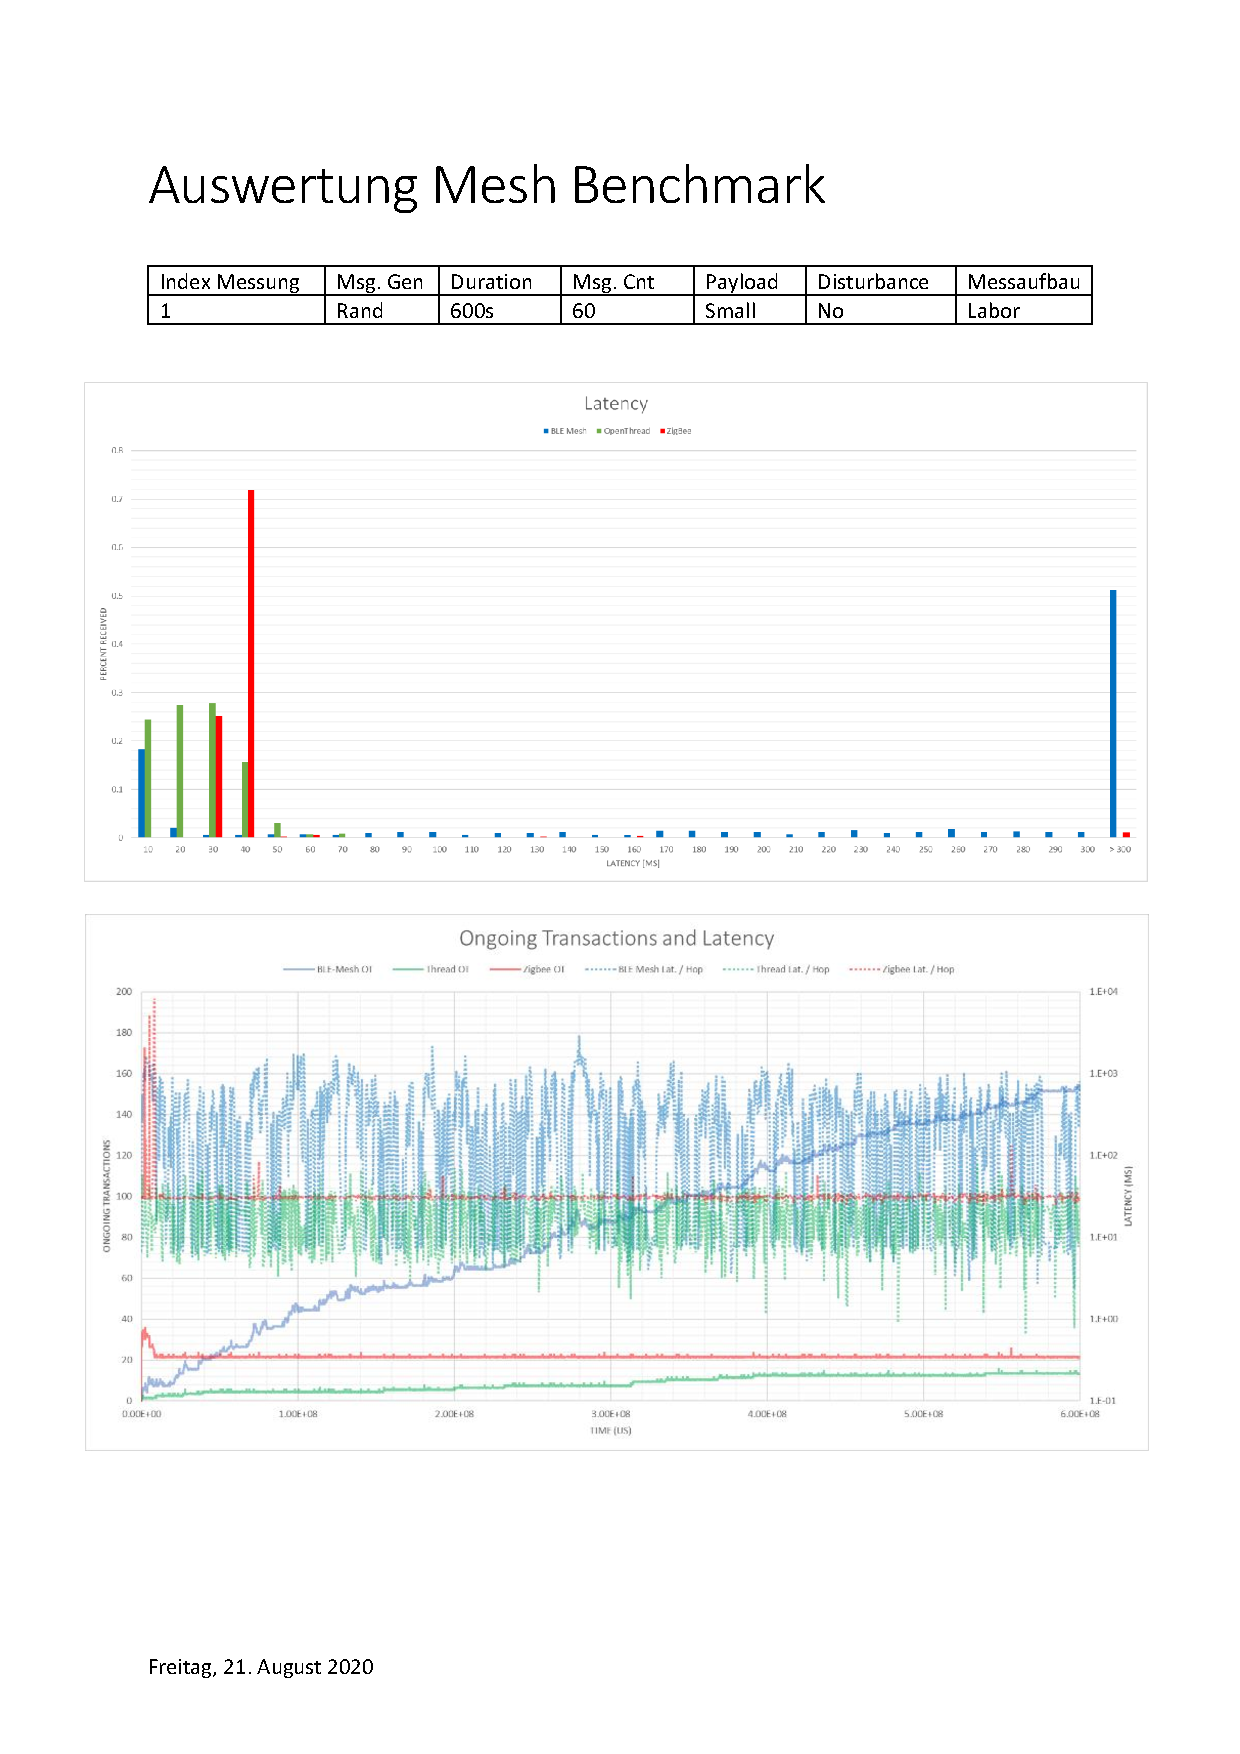
\includepdf[pages={1}, nup=1x1, landscape=false, scale=0.95 ,offset=0 -20, pagecommand={\section{Messprotokolle Mesh Benchmark}\label{app:MessprotokolleMeshBenchmark}\thispagestyle{myheadings}}]{appendix/Messprotokolle_Labor.pdf}

\includepdf[pages={2-14}, nup=1x1, landscape=false, scale=0.95 ,offset=0 0, pagecommand={\thispagestyle{myheadings}}]{appendix/Messprotokolle_Labor.pdf}

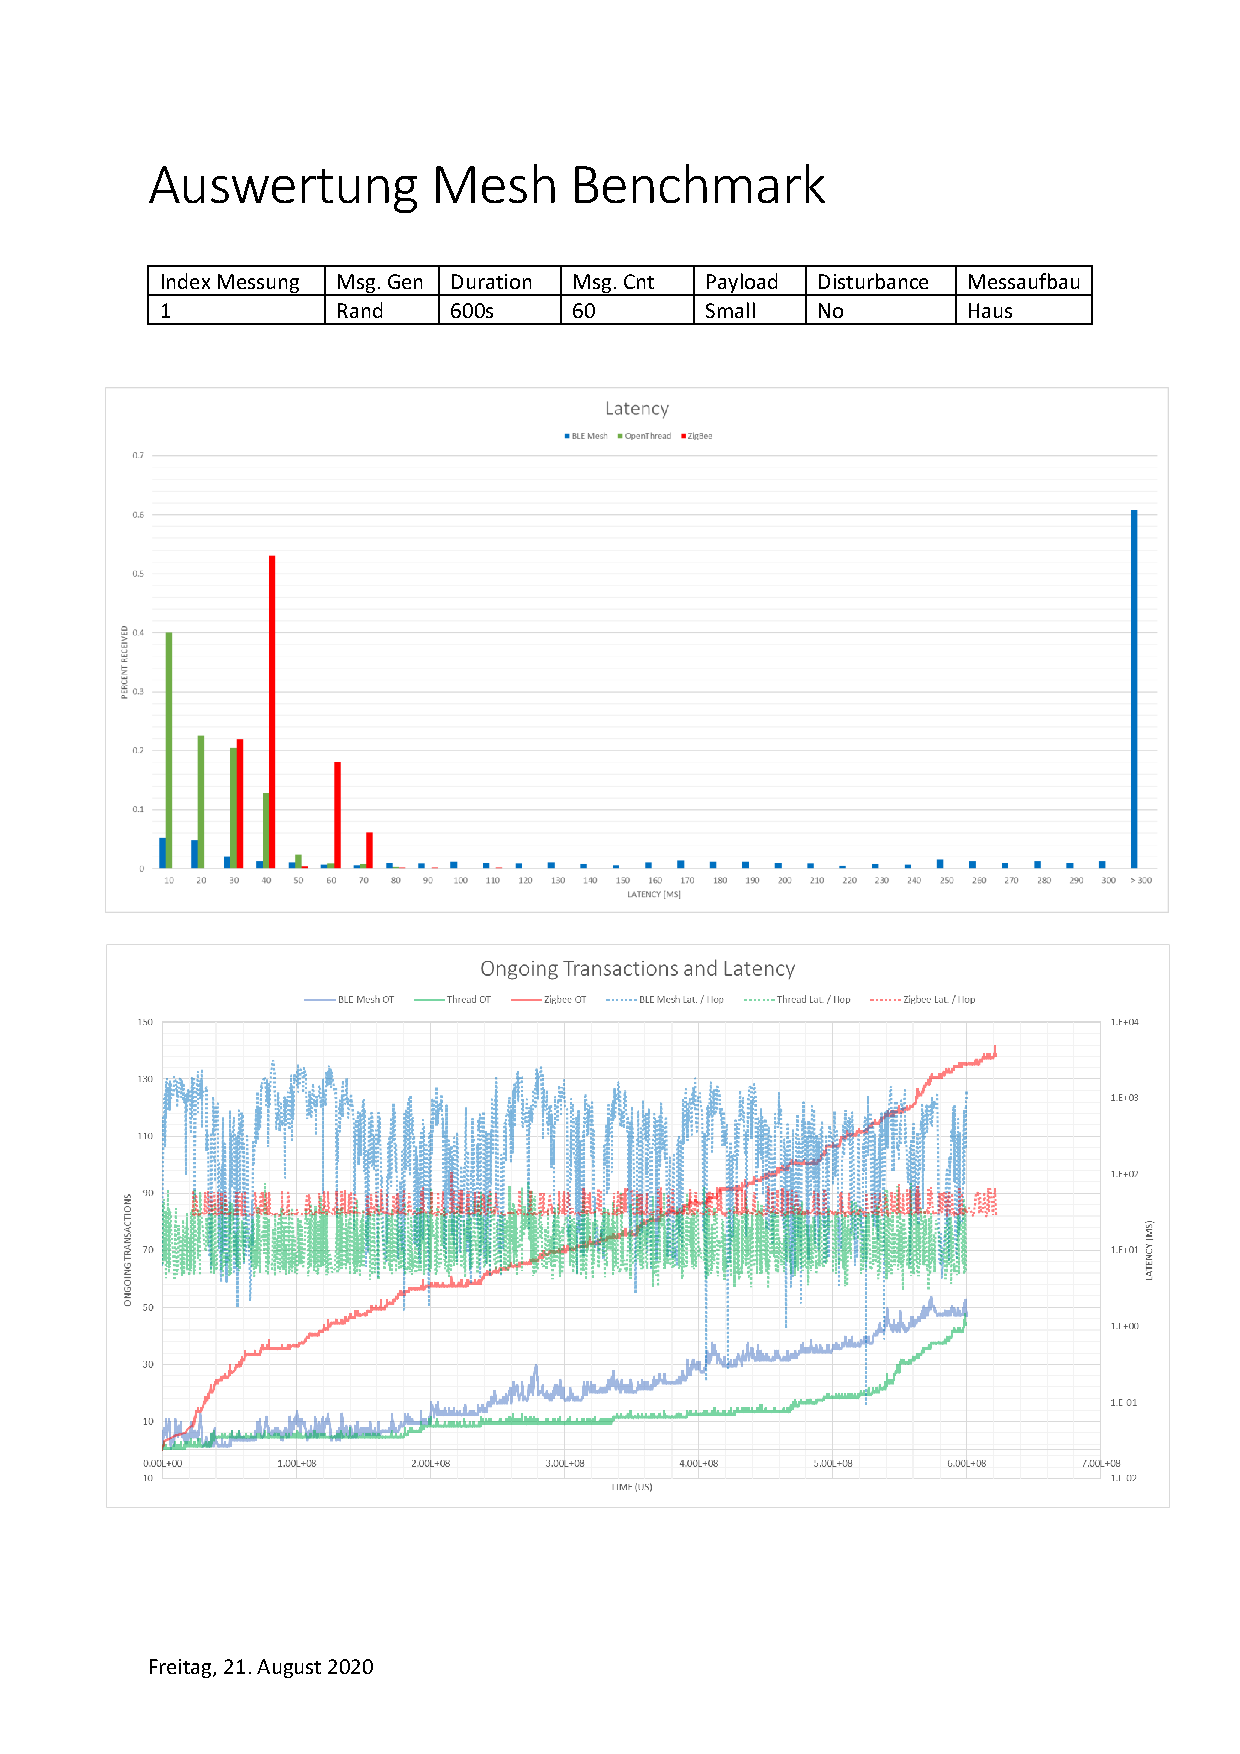
\includepdf[pages={1}, nup=1x1, landscape=false, scale=0.95 ,offset=0 0, pagecommand={\thispagestyle{myheadings}}]{appendix/Messprotokolle_Haus.pdf}

\includepdf[pages={2-8}, nup=1x1, landscape=false, scale=0.95 ,offset=0 0, pagecommand={\thispagestyle{myheadings}}]{appendix/Messprotokolle_Haus.pdf}

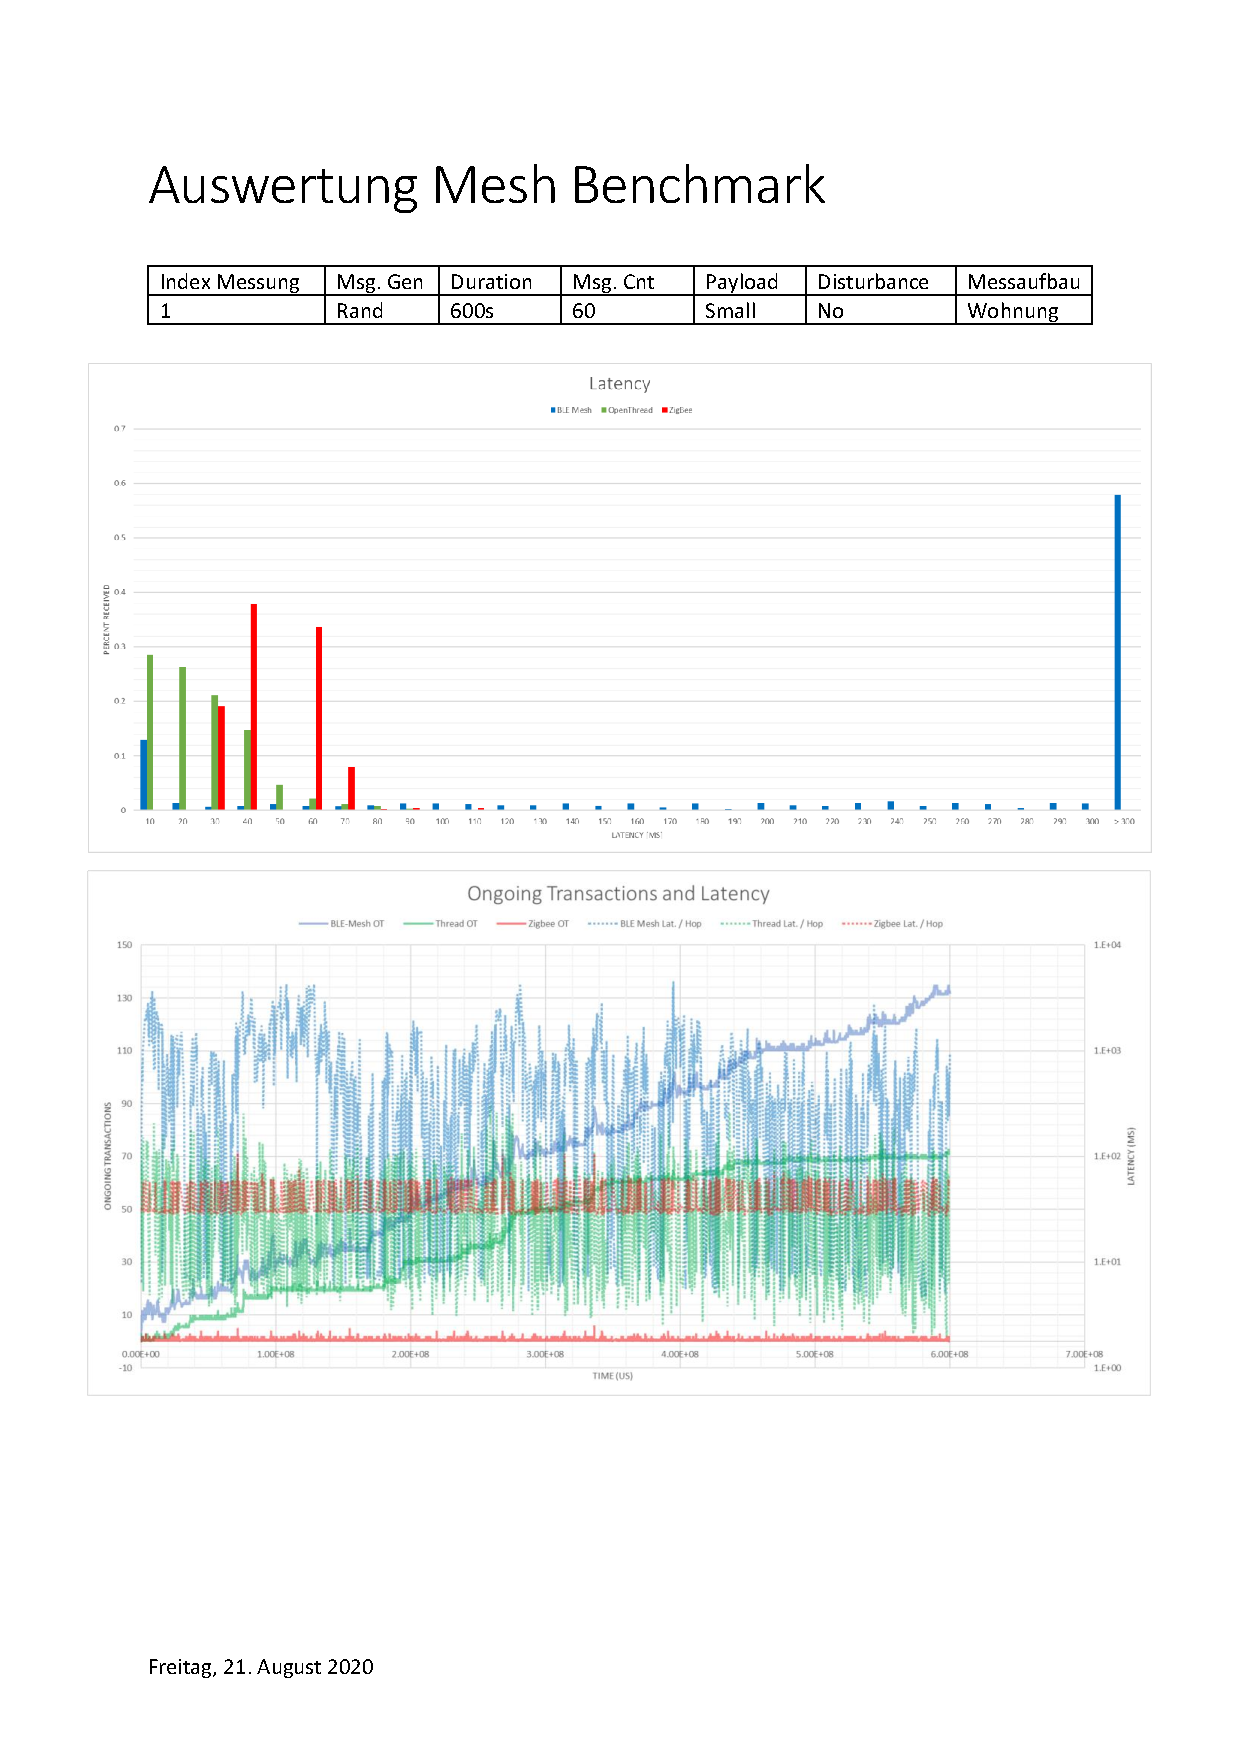
\includepdf[pages={1}, nup=1x1, landscape=false, scale=0.95 ,offset=0 0, pagecommand={\thispagestyle{myheadings}}]{appendix/Messprotokolle_Wohnung.pdf}

\includepdf[pages={2-8}, nup=1x1, landscape=false, scale=0.95 ,offset=0 0, pagecommand={\thispagestyle{myheadings}}]{appendix/Messprotokolle_Wohnung.pdf}

%***************Random Value Generation*********************
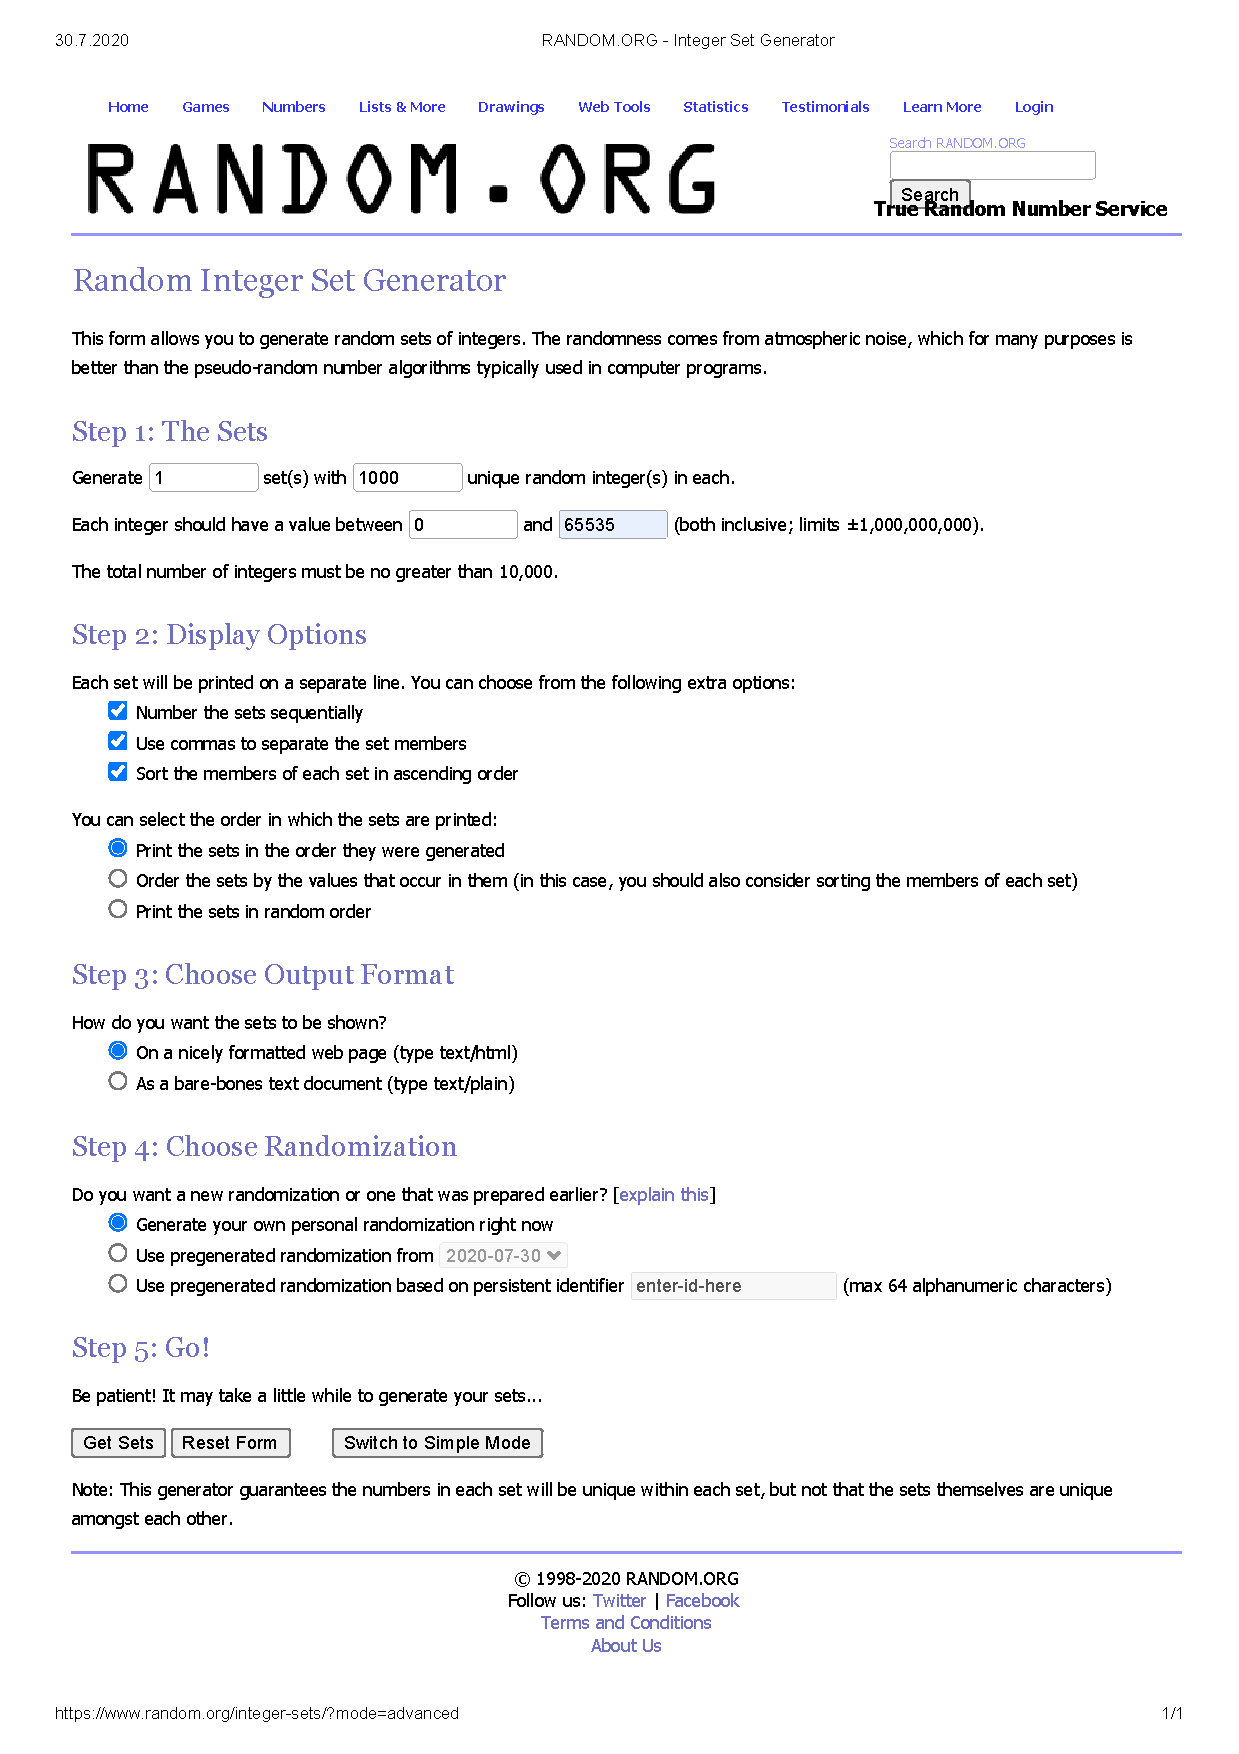
\includepdf[pages={1}, nup=1x1, landscape=false, scale=0.8 ,offset=0 -20, pagecommand={\section{Random Traffic Generation}\label{app:RandomTrafficGeneration}\thispagestyle{myheadings}}]{appendix/RANDOM.ORG_Integer_Set_Generator.pdf}


\end{appendix}



%%---NOTES for DEBUG---------------------------------------------------------------------
\ifdraft{%Do this only if mode=draft
%%requires \usepackage{todonotes})
\newpage
\listoftodos[\section{Todo-Notes}]
\clearpage
}
{%Do this only if mode=final
}

\end{document}
